\documentclass[12pt]{article}
\usepackage[utf8]{inputenc}
\usepackage[brazil]{babel}
\usepackage{graphicx}
\usepackage{amsmath}
\usepackage{hyperref}
\usepackage{caption}
\usepackage{geometry}
\usepackage{enumitem}
\usepackage{booktabs}
\usepackage{multirow}
\usepackage{colortbl}
\usepackage{xcolor}
\usepackage{subcaption}
\usepackage{tikz,tikz-3dplot} 
\usepackage[linesnumbered,ruled,vlined]{algorithm2e}

\geometry{a4paper, margin=2.5cm}
\setlength { \parskip }{0.3\baselineskip }

\hypersetup{
    colorlinks=true,
    linkcolor=black,
    citecolor=black,
    urlcolor=black
}


%=======================================================
%  INDIQUE AQUI O NOME DO PROBLEMA E A EQUIPE 
%=======================================================
\title{Universidade Federal de Juiz de Fora \\
        DCC059 - Teoria dos Grafos \\
        \vspace{6.0cm}
        {\Huge\textbf{Nome do Problema \\
                      Abordado}}\\
        \vspace{6.0cm}
}
\author{
    Nome do Aluno 1 - Matricula: \\
    Nome do Aluno 2 - Matricula: \\
    Nome do Aluno 3 - Matricula: \\
    Nome do Aluno 4 - Matricula: \\
}
\date{Dezembro de 2026}





%=======================================================
%=======================================================
\begin{document}

\maketitle
\newpage

\tableofcontents
\newpage

%=======================================================
%                 I N T R O D U Ç Ã O
%=======================================================
\section{Introdução}

\colorbox{pink}{
\begin{minipage}[c]{14cm}
[\textbf{Atenção}:] o relatório deve ter no máximo \textbf{10 páginas},
sem contar capa, sumário e bibliografia, e \textbf{não} deve conter
código-fonte. Apague todas as instruções deste modelo antes de entregar.
\end{minipage} }

O presente relatório tem como objetivo $\dots$. Considerou-se neste trabalho as características do problema  $\dots$. Foram desenvolvidos três algoritmos construtivos:  um algoritmo guloso, um guloso randomizado e um guloso randomizado reativo, que foram avaliados sobre um conjunto de instâncias e os resultados foram comparados com os apresentados em citar.

Note que nesta seção você deve dar uma visão geral do que consiste o trabalho, podendo destacar o contexto do mesmo no escopo da disciplina de Grafos, os objetivos e a motivação para o desenvolvimento do mesmo. O último parágrafo segue mais ou menos o modelo a seguir.

O restante do trabalho está assim estruturado: na Seção \ref{secProblema} o problema é descrito formalmente através de um modelo em grafos; a Seção \ref{secAlgoritmos} descreve as abordagens propostas para o problema, enquanto a Seção \ref{secResultados} apresenta os experimentos computacionais, onde se descreve o design dos experimentos, o conjunto de instâncias (\textit{benchmarks}), os testes de verificação da implementação e a análise comparativa dos resultados dos algoritmos desenvolvidos; a Seção \ref{secIA} descreve o uso de ferramentas de inteligência artificial; por fim, a Seção \ref{secConclusoes} traz as conclusões do trabalho e propostas de trabalhos futuros.



%=======================================================
%     D E S C R I Ç Ã O     D O    P R O B L E M A
%=======================================================
\section{Descrição do Problema}
\label{secProblema}

Dado um grafo \( G = (V, E) \) conexo, ... conforme descrito em \cite{}.

Nesta seção você deve descrever formalmente o problema modelado em grafos: o que é dado (o grafo e eventuais parâmetros), o que é uma solução viável e qual é a função objetivo. Segue um exemplo de como fazer isso para uma variação do problema da árvore geradora:

Uma solução viável é uma árvore geradora \( T = (V, E_T) \) de \( G \), isto é, um subgrafo com \( E_T \subseteq E \) que é conexo, acíclico e contém todos os vértices de \( G \) (e, portanto, \( |E_T| = |V| - 1 \)). Seja \( \delta_T(v) \) o grau do vértice \( v \) em \( T \). O problema consiste em encontrar uma árvore geradora \( T \) que
\begin{eqnarray}
\min ~ f(T) ~=~ \left|\{\, v \in V : \delta_T(v) > 2 \,\}\right| & & \label{func_obj}
\end{eqnarray}

A função objetivo (\ref{func_obj}) conta o número de vértices de grau maior que 2 na árvore $T$.

\textbf{Observação:} este é apenas um exemplo. Você pode, se quiser, apresentar também uma formulação de Programação Matemática, mas o essencial é que o problema seja descrito formalmente através de modelagem em grafos.

Ilustre sempre que possível e, sempre que inserir uma figura ou tabela, escreva algo que a explique. Como é possível observar na Figura \ref{fig:exemplo-imagem}, $\dots$.


\begin{figure}[h]
    \centering
    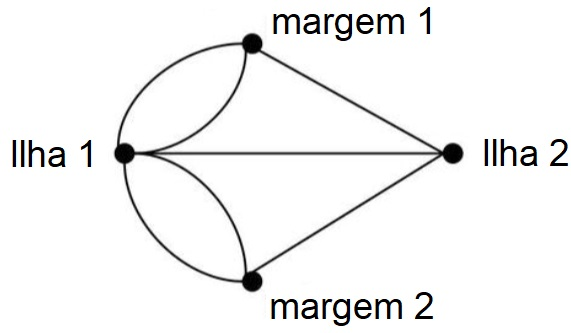
\includegraphics[width=0.3\textwidth]{img/Grafo-konigsberg.jpg} % substitua pelo nome do arquivo da sua imagem
    \caption{Essa figura é um arquivo jpg (Fonte: indique a referência de quem fez a figura)}
    \label{fig:exemplo-imagem}
\end{figure}

Se preferir, desenhe os grafos da instância e de uma solução para ilustrar melhor o problema.

\begin{figure}[ht!]
  \centering
  
  \begin{subfigure}{0.95\textwidth}
    \centering
    \begin{tikzpicture}
%============================================================
%  Essa seção define o estilo dos nós e arestas  
%  Necessário apenas para desenhar um grafo se quiserem
%============================================================
\tikzset{ % Importante:
          % Linha em branco nessa seção dá erro de compilação!
    % ESTILOS DOS GRAFOS
    % ---  Define arestas ------
    >=stealth,
    aresta/.style={ %
            -,     % sem terminação na aresta
            thick  % linha grossa
        },
    arco/.style={  % 
            ->,    % com seta no final da aresta
            thick  % linha grossa
        },
    outraAresta/.style={ -, %
            thin,  % linha fina
            dashed,% tracejada (dotted para pontilhada)
            gray   % cor da aresta 
        },
    % ---  Define vertices ------
    vertice/.style={   %
            circle,    % formato circular
            semithick, % linha "meio" grossa
            draw=black,% linha na cor preta
            inner sep=2pt % margem interna
        },
    verticeRetangular/.style={ %
            rectangle, % formato retangular
            very thick, % linha muito grossa
            draw=black  % linha na cor preta 
        },
    texto/.style={      %
            draw=white, % contorno em branco 
            font=\footnotesize %texto em letra pequena
        },
    % --- SOBRE CORES ------
    % Existem algumas cores padrão: blue, yellow, teal, 
    %     purple, red, violet, white, gray, lightgray...
    % As cores originais (principalmente blue, red, green)
    % são muito vivas, mas podem ser "diluidas": 
    %   blue!30         => 30% de azul com 70% de branco
    %   blue!80!black   => 80% de azul com 20% de preto
}


   % insere um nó com o estilo "vertice" (definido nas linhas 6 a 40 do arquivo)
   %    que será referenciado por v1 na posicao (x,y) do plano cartesiano indicada 
   %    com o texto interno "1"
   \node[vertice] (v1) at (0.6,0.2) {\footnotesize 1};
   % insere o vertice, mudando a cor padrão para 60% vinho 40% branco 
   % (veja comentario sobre cores nas linhas 40-46) 
   \node[verticeRetangular,fill=purple!30] (v2) at (-0.5,1) {\footnotesize 2};
   \node[vertice] (v3) at (1,2.1) {\footnotesize 3};
   \node[vertice] (v4) at (2.8,1.9) {\footnotesize 4};
   \node[vertice] (v5) at (3.8,1) {\footnotesize 5};
   \node[verticeRetangular,fill=teal!30] (v6) at (3,0.2) {\footnotesize 6};
   \node[vertice] (v7) at (2,1) {\footnotesize 7};


   
   % insere uma aresta com o estilo "aresta" (definido nas linhas 6 a 40)
   %    do nó v1 ao nó v2, com um nó intermediario contendo o texto "a"
   %    Os termos below, above, right, left, near start, near end ajudam a 
   %    posicionar o texto na aresta
   \draw[aresta] (v1) edge node[below left] {\footnotesize a} (v2);
   \draw[aresta] (v1) edge node[near end, left] {\footnotesize c} (v3);
   \draw[aresta] (v1) edge node[below] {\footnotesize d} (v6);
   \draw[aresta] (v1) edge node[near end, below] {\footnotesize e} (v7);
   \draw[aresta] (v2) edge node[above] {\footnotesize b} (v3);
   \draw[aresta] (v2) edge node[very near end, above] {\footnotesize f} (v7);
   \draw[aresta] (v3) edge node[above] {\footnotesize g} (v4);
   \draw[aresta] (v4) edge node[near end, above] {\footnotesize h} (v5);
   \draw[outraAresta] (v4) edge node[near start, below] {\footnotesize i} (v7);
   \draw[outraAresta] (v5) edge node[near start, below] {\footnotesize k} (v6);
   \draw[outraAresta] (v6) edge node[near start, above] {\footnotesize j} (v7);


    % Legenda 
    \node[texto,anchor=north west] (titulolegenda) at (5,2.4) {Legenda:};  
    \node[verticeRetangular,fill=purple!30,anchor=north west] (leg1) at (5,1.8) {};
    \node[texto,anchor=north west] (leg1txt) at (5.3,1.9) {Nó de origem};
    \node[verticeRetangular,fill=teal!30,anchor=north west] (leg1) at (5,1.3) {};
    \node[texto,anchor=north west] (leg1txt) at (5.3,1.4) {Nó de destino};
    
    \draw[aresta] (4.7,2.45) -- (8,2.45) -- (8,0.5) -- (4.7,0.5) -- cycle;
\end{tikzpicture}
    \caption{Instância desenhada no arquivo grafo1 }
    \label{fig:grafo1}
  \end{subfigure}
  
\vspace{1cm} % espaço vertical de 1cm entre figura de cima e as de baixo
  \begin{subfigure}{0.45\textwidth}
    \centering
    % use resizebox se precisar reduzir ou aumentar uma figura
    \resizebox{0.9\textwidth}{!}{ 
    \begin{tikzpicture}


%============================================================
%  ESTILOS DO GRAFO
%============================================================
\tikzset{ % Importante:
          % Linha em branco nessa seção dá erro de compilação!
    % ESTILOS DOS GRAFOS
    % ---  Define arestas ------
    >=stealth,
    aresta/.style={ %
            -,     % sem terminação na aresta
            thick  % linha grossa
        },
    arco/.style={  % 
            ->,    % com seta no final da aresta
            thick  % linha grossa
        },
    outraAresta/.style={ -, %
            thin,  % linha fina
            dashed,% tracejada (dotted para pontilhada)
            gray   % cor da aresta 
        },
    % ---  Define vertices ------
    vertice/.style={   %
            circle,    % formato circular
            semithick, % linha "meio" grossa
            draw=black,% linha na cor preta
            inner sep=2pt % margem interna
        },
    verticeRetangular/.style={ %
            rectangle, % formato retangular
            very thick, % linha muito grossa
            draw=black  % linha na cor preta 
        },
    texto/.style={      %
            draw=white, % contorno em branco 
            font=\footnotesize %texto em letra pequena
        },
    % --- SOBRE CORES ------
    % Existem algumas cores padrão: blue, yellow, teal, 
    %     purple, red, violet, white, gray, lightgray...
    % As cores originais (principalmente blue, red, green)
    % são muito vivas, mas podem ser "diluidas": 
    %   blue!30         => 30% de azul com 70% de branco
    %   blue!80!black   => 80% de azul com 20% de preto
}


%============================================================
%  VERTICES DO GRAFO
%============================================================
   % insere um nó com o estilo "vertice" (definido nas linhas 6 a 40 do arquivo) que será referenciado por v1 na posicao (x,y) do plano cartesiano indicada com o texto interno "1"
   \node[vertice] (v1) at (0.6,0.2) {\footnotesize 1};
   
   % insere o vertice, mudando a cor padrão para 60% vinho 40% branco (veja comentario sobre cores nas linhas 40-46) 
   \node[verticeRetangular,fill=purple!40] (v2) at (-0.5,1) {\footnotesize 2};

   % insere os outros nós
   \node[vertice] (v3) at (1,2.1) {\footnotesize 3};
   \node[vertice] (v4) at (2.8,1.9) {\footnotesize 4};
   \node[vertice] (v5) at (3.8,1) {\footnotesize 5};
   \node[verticeRetangular,fill=teal!40] (v6) at (3,0.2) {\footnotesize 6};
   \node[vertice] (v7) at (2,1) {\footnotesize 7};


   
%============================================================
%  ARESTAS DO GRAFO
%============================================================
   % insere uma aresta com o estilo "aresta" (definido nas linhas 6 a 40) do nó v1 ao nó v6, com um rótulo na aresta contendo o texto "d"
   \draw[aresta] (v1) edge node[below] {\footnotesize d} (v6);
   % Os termos below, above, right, left, near start, near end ajudam a posicionar o texto na aresta
   \draw[aresta] (v1) edge node[near end, below] {\footnotesize e} (v7);
   \draw[aresta,gray,dotted] (v2) edge node[above] {\footnotesize b} (v3);
   \draw[aresta,blue] (v2) edge node[very near end, above] {\footnotesize f} (v7);
   \draw[aresta,red] (v3) edge node[above] {\footnotesize g} (v4);
   \draw[aresta] (v4) edge node[near end, above] {\footnotesize h} (v5)

\end{tikzpicture}
    }
    \caption{Grafo do arquivo grafo3}
    \label{fig:grafo2}
  \end{subfigure}
  \hfill
  \begin{subfigure}{0.45\textwidth}
    \centering
    % use resizebox se precisar reduzir ou aumentar uma figura
    \resizebox{0.9\textwidth}{!}{
    \begin{tikzpicture}


%============================================================
%  ESTILOS DO GRAFO
%============================================================
\tikzset{ % Importante:
          % Linha em branco nessa seção dá erro de compilação!
    % ESTILOS DOS GRAFOS
    % ---  Define arestas ------
    >=stealth,
    aresta/.style={ %
            -,     % sem terminação na aresta
            thick  % linha grossa
        },
    arco/.style={  % 
            ->,    % com seta no final da aresta
            thick  % linha grossa
        },
    outraAresta/.style={ -, %
            thin,  % linha fina
            dashed,% tracejada (dotted para pontilhada)
            gray   % cor da aresta 
        },
    % ---  Define vertices ------
    vertice/.style={   %
            circle,    % formato circular
            semithick, % linha "meio" grossa
            draw=black,% linha na cor preta
            inner sep=2pt % margem interna
        },
    verticeRetangular/.style={ %
            rectangle, % formato retangular
            very thick, % linha muito grossa
            draw=black  % linha na cor preta 
        },
    texto/.style={      %
            draw=white, % contorno em branco 
            font=\footnotesize %texto em letra pequena
        },
    % --- SOBRE CORES ------
    % Existem algumas cores padrão: blue, yellow, teal, 
    %     purple, red, violet, white, gray, lightgray...
    % As cores originais (principalmente blue, red, green)
    % são muito vivas, mas podem ser "diluidas": 
    %   blue!30         => 30% de azul com 70% de branco
    %   blue!80!black   => 80% de azul com 20% de preto
}


%============================================================
%  VERTICES DO GRAFO
%============================================================
   % insere um nó com o estilo "vertice" (definido nas linhas 6 a 40 do arquivo) que será referenciado por v1 na posicao (x,y) do plano cartesiano indicada com o texto interno "1"
   \node[vertice] (v1) at (0.6,0.2) {\footnotesize 1};
   
   % insere o vertice, mudando a cor padrão para 60% vinho 40% branco (veja comentario sobre cores nas linhas 40-46) 
   \node[verticeRetangular,fill=purple!40] (v2) at (-0.5,1) {\footnotesize 2};

   % insere os outros nós
   \node[vertice] (v3) at (1,2.1) {\footnotesize 3};
   \node[vertice] (v4) at (2.8,1.9) {\footnotesize 4};
   \node[vertice] (v5) at (3.8,1) {\footnotesize 5};
   \node[verticeRetangular,fill=teal!40] (v6) at (3,0.2) {\footnotesize 6};
   \node[vertice] (v7) at (2,1) {\footnotesize 7};


   
%============================================================
%  ARESTAS DO GRAFO
%============================================================
   % insere uma aresta com o estilo "aresta" (definido nas linhas 6 a 40) do nó v1 ao nó v6, com um rótulo na aresta contendo o texto "d"
   \draw[aresta] (v1) edge node[below] {\footnotesize d} (v6);
   % Os termos below, above, right, left, near start, near end ajudam a posicionar o texto na aresta
   \draw[aresta] (v1) edge node[near end, below] {\footnotesize e} (v7);
   \draw[aresta,gray,dotted] (v2) edge node[above] {\footnotesize b} (v3);
   \draw[aresta,blue] (v2) edge node[very near end, above] {\footnotesize f} (v7);
   \draw[aresta,red] (v3) edge node[above] {\footnotesize g} (v4);
   \draw[aresta] (v4) edge node[near end, above] {\footnotesize h} (v5)

\end{tikzpicture}
    }
    \caption{Repeti para mostrar como colocar lado a lado}
    \label{fig:grafo2-ladoalado}
  \end{subfigure}
  
  \caption{O arquivo grafo3 está bem comentado, para que vocês possam adaptar facilmente o desenho para outros grafos}
  \label{fig:acima}
\end{figure}

Os exemplos de grafos incluídos nos arquivos têm estilos diferentes para ilustrar diferentes possibilidades, caso queiram utilizar esse recurso. Outros exemplos de grafos podem ser encontrados em \href{https://tikz.net}{Tikz.net} ou em \href{https://texample.net}{TeXample.net}.



%=======================================================
%                 A L G O R I T M O S
%=======================================================
\section{Algoritmos Implementados}
\label{secAlgoritmos}

Nesta seção são detalhados os algoritmos propostos para a obtenção de soluções para o problema xyz.
É importante que os algoritmos sejam apresentados de forma detalhada, de forma que seja possível que qualquer pessoa consiga reproduzir os algoritmos propostos. 

\subsection{Algoritmo Guloso}
\label{subSecAlgGuloso}

Descrever o algoritmo guloso, colocando também o pseudocódigo. Vide exemplo no Algoritmo \ref{algGuloso}. Lembre-se de descrever o algoritmo apresentado, a numeração das linhas pode ajudar nesta explicação. Os algoritmos não são autoexplicativos, você precisa direcionar o leitor na leitura do pseudocódigo.

\begin{algorithm}[H]
\caption{Algoritmo Guloso}
\label{algGuloso}
\KwIn{Grafo \( G = (V, E) \)}
\KwOut{Árvore geradora $T$}

$T \leftarrow \emptyset$\;
\While{$T$ não é uma solução completa}{
    Exemplo de algoritmo\;
}
\Return{$T$}
\end{algorithm}

Pode ser interessante destacar as limitações do algoritmo proposto, destacando os cenários onde é mais difícil para o algoritmo obter boas soluções. 


\subsection{Algoritmo Guloso Randomizado}
\label{subSecAlgRand}

Descrever o algoritmo guloso randomizado, justificar a proposta do mesmo sobre as limitações da abordagem gulosa descrita na seção anterior e colocar também o pseudocódigo.


\subsection{Algoritmo Guloso Randomizado Reativo}
\label{subSecAlgRandReact}
Descrever o algoritmo guloso randomizado reativo, justificar a proposta do mesmo sobre as limitações da abordagem gulosa randomizada descrita na seção anterior e colocar também o pseudocódigo.

\begin{figure}[ht]
\centering
\resizebox{0.5\textwidth}{!}{
    % Exemplo de diagrama disponivel em https://texample.net/android/
% Diagram of Android activity life cycle
% Author: Pavel Seda 
\usetikzlibrary{arrows.meta}
\tikzset{%
  >={Latex[width=2mm,length=2mm]},
  % Specifications for style of nodes:
            base/.style = {rectangle, rounded corners, draw=black,
                           minimum width=4cm, minimum height=1cm,
                           text centered, font=\sffamily},
  activityStarts/.style = {base, fill=blue!30},
       startstop/.style = {base, fill=red!30},
    activityRuns/.style = {base, fill=green!30},
         process/.style = {base, minimum width=2.5cm, fill=orange!15,
                           font=\ttfamily},
}
% Drawing part, node distance is 1.5 cm and every node
% is prefilled with white background
\begin{tikzpicture}[node distance=1.5cm,
    every node/.style={fill=white, font=\sffamily}, align=center]
  % Specification of nodes (position, etc.)
  \node (start)             [activityStarts]              {Activity starts};
  \node (onCreateBlock)     [process, below of=start]          {onCreate()};
  \node (onStartBlock)      [process, below of=onCreateBlock]   {onStart()};
  \node (onResumeBlock)     [process, below of=onStartBlock]   {onResume()};
  \node (activityRuns)      [activityRuns, below of=onResumeBlock]
                                                      {Activity is running};
  \node (onPauseBlock)      [process, below of=activityRuns, yshift=-1cm]
                                                                {onPause()};
  \node (onStopBlock)       [process, below of=onPauseBlock, yshift=-1cm]
                                                                 {onStop()};
  \node (onDestroyBlock)    [process, below of=onStopBlock, yshift=-1cm] 
                                                              {onDestroy()};
  \node (onRestartBlock)    [process, right of=onStartBlock, xshift=4cm]
                                                              {onRestart()};
  \node (ActivityEnds)      [startstop, left of=activityRuns, xshift=-4cm]
                                                        {Process is killed};
  \node (ActivityDestroyed) [startstop, below of=onDestroyBlock]
                                                    {Activity is shut down};     
  % Specification of lines between nodes specified above
  % with aditional nodes for description 
  \draw[->]             (start) -- (onCreateBlock);
  \draw[->]     (onCreateBlock) -- (onStartBlock);
  \draw[->]      (onStartBlock) -- (onResumeBlock);
  \draw[->]     (onResumeBlock) -- (activityRuns);
  \draw[->]      (activityRuns) -- node[text width=4cm]
                                   {Another activity comes in
                                    front of the activity} (onPauseBlock);
  \draw[->]      (onPauseBlock) -- node {The activity is no longer visible}
                                   (onStopBlock);
  \draw[->]       (onStopBlock) -- node {The activity is shut down by
                                   user or system} (onDestroyBlock);
  \draw[->]    (onRestartBlock) -- (onStartBlock);
  \draw[->]       (onStopBlock) -| node[yshift=1.25cm, text width=3cm]
                                   {The activity comes to the foreground}
                                   (onRestartBlock);
  \draw[->]    (onDestroyBlock) -- (ActivityDestroyed);
  \draw[->]      (onPauseBlock) -| node(priorityXMemory)
                                   {higher priority $\rightarrow$ more memory}
                                   (ActivityEnds);
  \draw           (onStopBlock) -| (priorityXMemory);
  \draw[->]     (ActivityEnds)  |- node [yshift=-2cm, text width=3.1cm]
                                    {User navigates back to the activity}
                                    (onCreateBlock);
  \draw[->] (onPauseBlock.east) -- ++(2.6,0) -- ++(0,2) -- ++(0,2) --                
     node[xshift=1.2cm,yshift=-1.5cm, text width=2.5cm]
     {The activity comes to the foreground}(onResumeBlock.east);
  \end{tikzpicture}
}
\caption{Exemplo imagem}
\label{fig:fluxograma}
\end{figure}

\textbf{Além do} pseudocódigo, você também pode acrescentar uma figura com um fluxograma, como na Figura \ref{fig:fluxograma}.




%=======================================================
%                 E X P E R I M E N T O S 
%=======================================================
\section{Experimentos computacionais}
\label{secResultados}
Nesta seção você deve descrever todo o experimento computacional. Para tanto, defina subseções.

\subsection{Descrição das instâncias}
\label{subSecInstancias}
Descreva as instâncias citando a referência onde as mesmas foram obtidas, se você testou apenas um subconjunto de instâncias da referência, explique qual(is) o(s) critério(s) utilizado(s) para a seleção do conjunto de instâncias usadas. Você pode listar as instâncias em uma tabela como no exemplo da Tabela \ref{tabInstancias}. E note que para o seu problema não necessariamente você terá todas essas colunas.

\begin{table}[!h]
\centering
\caption{Exemplo de tabela com descrição das instâncias}
\begin{tabular}{|l|c|c|c|c|}
\hline
\multicolumn{1}{|c|}{\textbf{Instância}} & \multicolumn{1}{c|}{\textbf{Núm Arestas}} & \multicolumn{1}{c|}{\textbf{Núm Vértices}} & \multicolumn{1}{c|}{\textbf{$K$}} & \multicolumn{1}{c|}{\textbf{$L$}}  \\ \hline
st323\_70a & 323 & 70 & 14 & 9   \\ \hline
proB789\_100a & 789 & 100 & 20 & 10  \\ \hline
lin884\_318 & 884 & 118 & 64 & 10   \\ \hline \hline
pcb2208\_442 & 2.208  & 442 & 89 & 10  \\ \hline
pr5314 & 5.314 & 439 & 88 & 10  \\ \hline
wath4180 & 4.180 & 699 & 20 & 25\\ \hline
lin41817\_710 & 41.817 & 710 & 21 & 25  \\ \hline \hline
kro121002 & 121.002 & 1.000 & 120 & 25  \\ \hline
dilc & 91.217 & 2.620 & 153 & 250  \\ \hline
pro789\_100a & 117.890 & 3.200 & 200 & 107  \\ \hline
\end{tabular}
\label{tabInstancias}
\end{table}


\subsection{Ambiente computacional e  parâmetros}
\label{subSecAmbiente}
Descreva o ambiente computacional utilizado citando a linguagem de programação, o compilador utilizado, o processador da máquina utilizada nos testes, o gerador de números aleatórios etc).

Descreva o conjunto de parâmetros usado (número de iterações, os três valores de $\alpha$ utilizados nos testes com o algoritmo guloso randomizado e a justificativa da escolha, os valores de $\alpha$ e o tamanho do bloco de atualização das probabilidades adotados no algoritmo guloso randomizado reativo etc.). Informe também que cada algoritmo foi executado 10 vezes para cada instância e cada valor de $\alpha$, com sementes diferentes.

\subsection{Verificação da implementação}
\label{subSecVerificacao}

Esta subseção é \textbf{obrigatória}. Descreva:
\begin{itemize}
    \item o \textbf{verificador} implementado: o que ele confere na solução (por exemplo: se é uma árvore, se usa apenas arestas do grafo, etc) e como o valor da função objetivo é recalculado;
    \item as \textbf{instâncias pequenas} construídas pelo grupo para testar os algoritmos, com a solução ótima obtida à mão (ilustre com figuras);
    
\begin{figure}[ht!]
  \centering
  \begin{subfigure}{0.45\textwidth}
    \centering
    % use resizebox se precisar reduzir ou aumentar uma figura
    \resizebox{0.9\textwidth}{!}{ 
    \begin{tikzpicture}


%============================================================
%  ESTILOS DO GRAFO
%============================================================
\tikzset{ % Importante:
          % Linha em branco nessa seção dá erro de compilação!
    % ESTILOS DOS GRAFOS
    % ---  Define arestas ------
    >=stealth,
    aresta/.style={ %
            -,     % sem terminação na aresta
            thick  % linha grossa
        },
    arco/.style={  % 
            ->,    % com seta no final da aresta
            thick  % linha grossa
        },
    outraAresta/.style={ -, %
            thin,  % linha fina
            dashed,% tracejada (dotted para pontilhada)
            gray   % cor da aresta 
        },
    % ---  Define vertices ------
    vertice/.style={   %
            circle,    % formato circular
            semithick, % linha "meio" grossa
            draw=black,% linha na cor preta
            inner sep=2pt % margem interna
        },
    verticeRetangular/.style={ %
            rectangle, % formato retangular
            very thick, % linha muito grossa
            draw=black  % linha na cor preta 
        },
    texto/.style={      %
            draw=white, % contorno em branco 
            font=\footnotesize %texto em letra pequena
        },
    % --- SOBRE CORES ------
    % Existem algumas cores padrão: blue, yellow, teal, 
    %     purple, red, violet, white, gray, lightgray...
    % As cores originais (principalmente blue, red, green)
    % são muito vivas, mas podem ser "diluidas": 
    %   blue!30         => 30% de azul com 70% de branco
    %   blue!80!black   => 80% de azul com 20% de preto
}


%============================================================
%  VERTICES DO GRAFO
%============================================================
   % insere um nó com o estilo "vertice" (definido nas linhas 6 a 40 do arquivo) que será referenciado por v1 na posicao (x,y) do plano cartesiano indicada com o texto interno "1"
   \node[vertice] (v1) at (0.6,0.2) {\footnotesize 1};
   
   % insere o vertice, mudando a cor padrão para 60% vinho 40% branco (veja comentario sobre cores nas linhas 40-46) 
   \node[verticeRetangular,fill=purple!40] (v2) at (-0.5,1) {\footnotesize 2};

   % insere os outros nós
   \node[vertice] (v3) at (1,2.1) {\footnotesize 3};
   \node[vertice] (v4) at (2.8,1.9) {\footnotesize 4};
   \node[vertice] (v5) at (3.8,1) {\footnotesize 5};
   \node[verticeRetangular,fill=teal!40] (v6) at (3,0.2) {\footnotesize 6};
   \node[vertice] (v7) at (2,1) {\footnotesize 7};


   
%============================================================
%  ARESTAS DO GRAFO
%============================================================
   % insere uma aresta com o estilo "aresta" (definido nas linhas 6 a 40) do nó v1 ao nó v6, com um rótulo na aresta contendo o texto "d"
   \draw[aresta] (v1) edge node[below] {\footnotesize d} (v6);
   % Os termos below, above, right, left, near start, near end ajudam a posicionar o texto na aresta
   \draw[aresta] (v1) edge node[near end, below] {\footnotesize e} (v7);
   \draw[aresta,gray,dotted] (v2) edge node[above] {\footnotesize b} (v3);
   \draw[aresta,blue] (v2) edge node[very near end, above] {\footnotesize f} (v7);
   \draw[aresta,red] (v3) edge node[above] {\footnotesize g} (v4);
   \draw[aresta] (v4) edge node[near end, above] {\footnotesize h} (v5)

\end{tikzpicture}
    }
    \caption{Grafo do arquivo grafo3}
    \label{fig:grafo3a_secao4}
  \end{subfigure}
  \hfill
  \begin{subfigure}{0.45\textwidth}
    \centering
    % use resizebox se precisar reduzir ou aumentar uma figura
    \resizebox{0.9\textwidth}{!}{
    \begin{tikzpicture}


%============================================================
%  ESTILOS DO GRAFO
%============================================================
\tikzset{ % Importante:
          % Linha em branco nessa seção dá erro de compilação!
    % ESTILOS DOS GRAFOS
    % ---  Define arestas ------
    >=stealth,
    aresta/.style={ %
            -,     % sem terminação na aresta
            thick  % linha grossa
        },
    arco/.style={  % 
            ->,    % com seta no final da aresta
            thick  % linha grossa
        },
    outraAresta/.style={ -, %
            thin,  % linha fina
            dashed,% tracejada (dotted para pontilhada)
            gray   % cor da aresta 
        },
    % ---  Define vertices ------
    vertice/.style={   %
            circle,    % formato circular
            semithick, % linha "meio" grossa
            draw=black,% linha na cor preta
            inner sep=2pt % margem interna
        },
    verticeRetangular/.style={ %
            rectangle, % formato retangular
            very thick, % linha muito grossa
            draw=black  % linha na cor preta 
        },
    texto/.style={      %
            draw=white, % contorno em branco 
            font=\footnotesize %texto em letra pequena
        },
    % --- SOBRE CORES ------
    % Existem algumas cores padrão: blue, yellow, teal, 
    %     purple, red, violet, white, gray, lightgray...
    % As cores originais (principalmente blue, red, green)
    % são muito vivas, mas podem ser "diluidas": 
    %   blue!30         => 30% de azul com 70% de branco
    %   blue!80!black   => 80% de azul com 20% de preto
}


%============================================================
%  VERTICES DO GRAFO
%============================================================
   % insere um nó com o estilo "vertice" (definido nas linhas 6 a 40 do arquivo) que será referenciado por v1 na posicao (x,y) do plano cartesiano indicada com o texto interno "1"
   \node[vertice] (v1) at (0.6,0.2) {\footnotesize 1};
   
   % insere o vertice, mudando a cor padrão para 60% vinho 40% branco (veja comentario sobre cores nas linhas 40-46) 
   \node[verticeRetangular,fill=purple!40] (v2) at (-0.5,1) {\footnotesize 2};

   % insere os outros nós
   \node[vertice] (v3) at (1,2.1) {\footnotesize 3};
   \node[vertice] (v4) at (2.8,1.9) {\footnotesize 4};
   \node[vertice] (v5) at (3.8,1) {\footnotesize 5};
   \node[verticeRetangular,fill=teal!40] (v6) at (3,0.2) {\footnotesize 6};
   \node[vertice] (v7) at (2,1) {\footnotesize 7};


   
%============================================================
%  ARESTAS DO GRAFO
%============================================================
   % insere uma aresta com o estilo "aresta" (definido nas linhas 6 a 40) do nó v1 ao nó v6, com um rótulo na aresta contendo o texto "d"
   \draw[aresta] (v1) edge node[below] {\footnotesize d} (v6);
   % Os termos below, above, right, left, near start, near end ajudam a posicionar o texto na aresta
   \draw[aresta] (v1) edge node[near end, below] {\footnotesize e} (v7);
   \draw[aresta,gray,dotted] (v2) edge node[above] {\footnotesize b} (v3);
   \draw[aresta,blue] (v2) edge node[very near end, above] {\footnotesize f} (v7);
   \draw[aresta,red] (v3) edge node[above] {\footnotesize g} (v4);
   \draw[aresta] (v4) edge node[near end, above] {\footnotesize h} (v5)

\end{tikzpicture}
    }
    \caption{Outra vez}
    \label{fig:grafo3b_secao4}
  \end{subfigure}
  
  \caption{O arquivo grafo3 está bem comentado, para que vocês possam adaptar facilmente o desenho para outros grafos}
  \label{fig:grafo3_secao4}
\end{figure}

    \item a execução do algoritmo guloso, \textbf{passo a passo}, em uma dessas instâncias (por exemplo, com uma tabela que mostre a lista de candidatos e o elemento escolhido em cada iteração).
\end{itemize}

Todas as soluções usadas nas tabelas da Seção \ref{subSecResultados} devem ter sido aprovadas pelo verificador.


\subsection{Resultados obtidos}
\label{subSecResultados}

Apresente aqui os resultados quanto à qualidade (valor da função de otimização). Explique o significado das colunas da tabela. Nas tabelas a seguir, os valores 0,10, 0,30 e 0,50 são apenas exemplos: substitua-os pelos valores de $\alpha$ escolhidos pelo grupo. Lembre-se de pôr em negrito os valores associados aos melhores resultados para cada instância. A Tabela \ref{tabResultExemplo} é um exemplo de apresentação dos resultados.

\begin{table}[htbp]
\centering
\caption{Resultados comparativos da melhor solução alcançada por cada algoritmo — diferença percentual em relação à melhor solução conhecida}
\renewcommand{\arraystretch}{1.2}
{
\footnotesize
\begin{tabular}{|c|c|c|c|c|c|c|c|}
\hline
\textbf{Instância} & \textbf{Melhor} & \textbf{Literatura} & \textbf{Guloso} & \multicolumn{3}{c|}{\textbf{Randomizado}} & \textbf{Reativo} \\ \cline{5-7}
 & & & &  \multicolumn{1}{c|}{{\bf 0,10}} & \multicolumn{1}{c|}{{\bf 0,30}} & \multicolumn{1}{c|}{{\bf 0,50}} & \\
\hline
I1 & 100 & \textbf{0,00} & 0,20 & 0,07 &  0,12 & \textbf{0,00} & 0,01 \\
I2 & 184 & 0,12 & \textbf{0,00} & 0,21 & 0,28 & 0,20 & \textbf{0,00} \\
\vdots & \vdots & \vdots & \vdots  & \vdots & \vdots & \vdots & \vdots \\
I10 &  &  &  &  &  &  &  \\
\hline
\textbf{Média} &  &  &  &  &  &  &  \\
\hline
\end{tabular}
}
\label{tabResultExemplo}
\end{table}

Segue um exemplo superficial de análise de resultados a partir de uma tabela:

Analisando a Tabela \ref{tabResultExemplo2}, é possível verificar que o algoritmo guloso randomizado com $\alpha = 0{,}10$ obteve os menores desvios na maioria das instâncias. Os maiores desvios do algoritmo guloso ocorreram nas instâncias mais densas, o que sugere que o critério guloso adotado é menos eficaz quando os vértices têm muitos vizinhos.

[\textit{Outro exemplo}] A Tabela \ref{tabResultExemplo2} mostra que, em relação à qualidade da solução, os algoritmos propostos não foram capazes de alcançar as melhores soluções conhecidas. Entretanto, comparando-se os resultados obtidos pelos algoritmos implementados, é possível perceber que o algoritmo Randomizado Reativo obteve um desempenho superior em 90\% das instâncias, especialmente nas instâncias compostas por grafos densos (observe que para imprimir \% é necessário usar uma barra invertida antes).

\colorbox{pink}{
\begin{minipage}[c]{13cm}
[\textbf{Nota}:] Nesta seção você precisa descrever os resultados, não apenas apresentar as tabelas. Procure destacar quais os melhores algoritmos, destacar se há alguma característica de uma ou mais instâncias (tamanho da instância, densidade de arestas ou grupo de instância específico) que esteja influenciando o comportamento de um ou outro algoritmo etc. 
\end{minipage} }

Além da Tabela \ref{tabResultExemplo} (que deve apresentar o desvio percentual dos melhores resultados alcançados por cada algoritmo), uma tabela semelhante deve ser utilizada para apresentar o desvio percentual da média dos resultados alcançados por cada algoritmo. Isso é, na Tabela \ref{tabResultExemplo}, o valor da melhor solução alcançada é utilizado para calcular os desvios e, na Tabela \ref{tabResultExemplo2}, a média dos valores das melhores soluções obtidas nas 10 execuções do algoritmo (para cada instância e cada valor de $\alpha$) deve ser utilizada nos cálculos do desvio percentual.


\begin{table}[htbp]
\centering
\caption{Resultados comparativos da média das soluções alcançadas nas 10 execuções de cada algoritmo — diferença percentual em relação à melhor solução conhecida}
\renewcommand{\arraystretch}{1.2}
{
\footnotesize
\begin{tabular}{|c|c|c|c|c|c|c|}
\hline
\textbf{Instância} & \textbf{Melhor} & \textbf{Guloso} & \multicolumn{3}{c|}{\textbf{Randomizado}} & \textbf{Reativo} \\ \cline{4-6}
 & & &  \multicolumn{1}{c|}{{\bf 0,10}} & \multicolumn{1}{c|}{{\bf 0,30}} & \multicolumn{1}{c|}{{\bf 0,50}} & \\
\hline
I1 & 100 & 0,20 & 0,07 &  0,12 & \textbf{0,00} & 0,01 \\
I2 & 184 & \textbf{0,00} & 0,21 &  0,28 & 0,20 & \textbf{0,00} \\
\vdots & \vdots & \vdots &  \vdots & \vdots & \vdots & \vdots \\
I10 &  &  &  &  &  &  \\
\hline
\textbf{Média} &  &  &  &  &  &  \\
\hline
\end{tabular}
}
\label{tabResultExemplo2}
\end{table}


A Tabela \ref{tabResultExemplo} e a Tabela \ref{tabResultExemplo2} são semelhantes, mas a Tabela \ref{tabResultExemplo} contém a coluna \textbf{Literatura}, que foi omitida na Tabela \ref{tabResultExemplo2}. A coluna \textbf{Literatura} só deve ser usada se houver resultados de \textbf{heurísticas} da literatura para as instâncias testadas; caso contrário, remova-a e use, nas duas tabelas, o modelo da Tabela \ref{tabResultExemplo2}.

Inclua ainda uma outra tabela com os dados  referentes ao tempo de processamento dos algoritmos. 


\begin{table}[htbp]
\centering
\caption{Tempo médio de execução de cada algoritmo (em seg)}
\renewcommand{\arraystretch}{1.2}
{
\footnotesize
\begin{tabular}{|c|c|c|c|c|c|}
\hline
\textbf{Instância} & \textbf{Guloso} & \multicolumn{3}{c|}{\textbf{Randomizado}} & \textbf{Reativo} \\ \cline{3-5}
 & &  \multicolumn{1}{c|}{{\bf 0,10}} & \multicolumn{1}{c|}{{\bf 0,30}} & \multicolumn{1}{c|}{{\bf 0,50}} & \\
\hline
I1 & 0,20 & 0,07 &  0,12 & 0,19 & 0,52 \\
I2 & 0,27 & 0,09 &  0,18 & 0,25 & 1,49 \\
\vdots &  \vdots & \vdots & \vdots & \vdots &  \vdots \\
I10 &  &  &  &  &  \\
\hline
\textbf{Média} &  &  &  &  &  \\
\hline
\end{tabular}
}
\label{tabResultTempo}
\end{table}

Lembre-se que é necessário analisar os dados de cada uma das tabelas!

%=======================================================
%           U S O   D E   I N T E L I G Ê N C I A   A R T I F I C I A L
%=======================================================
\section{Uso de ferramentas de inteligência artificial}
\label{secIA}

Esta seção é \textbf{obrigatória}. Descreva, de forma sucinta:
\begin{itemize}
    \item se o grupo usou ferramentas de IA e quais;
    \item para quais tarefas (por exemplo: geração de código, depuração, dúvidas de C++, revisão do texto);
    \item como o grupo verificou a corretude do que foi produzido com o auxílio da IA.
\end{itemize}
Caso o grupo não tenha usado IA, declare isso explicitamente.

%=======================================================
%                 C O N C L U S Õ E S
%=======================================================
\section{Conclusões}
\label{secConclusoes}

Apresente aqui as conclusões do trabalho. Comece descrevendo um resumo sucinto do que consistiu o trabalho, o problema modelado em grafos, o que foi implementado. Se tiver sugestões de melhorias para os algoritmos propostos, apresente aqui. Apresente também as principais dificuldades encontradas durante a realização do trabalho 2.



%=======================================================
%             R E F E R Ê N C I A S
%=======================================================
% Incluindo referências bibliográficas
% ATENCAO: as referências incluidas no arquivo bibliografia.bib só aparecem no documento quando efetivamente citadas no texto.
\bibliographystyle{plain} %define o estilo    
\bibliography{bibliografia} %busca o arquivo


\end{document}